% Created 2014-10-01 Wed 19:50
\documentclass[aps,prb,citeautoscript,preprint,citeautoscript,showkeys]{revtex4-1}
  \usepackage{graphicx}
\usepackage{subfigure}
\date{\today}
\title{blog}
\begin{document}

\section{redefining how images are displayed}
\label{sec-1}

\begin{minted}[frame=lines,fontsize=\scriptsize,linenos]{common-lisp}
(defun org-display-inline-images (&optional include-linked refresh beg end)
  "Display inline images.
Normally only links without a description part are inlined, because this
is how it will work for export.  When INCLUDE-LINKED is set, also links
with a description part will be inlined.  This can be nice for a quick
look at those images, but it does not reflect what exported files will look
like.
When REFRESH is set, refresh existing images between BEG and END.
This will create new image displays only if necessary.
BEG and END default to the buffer boundaries."
  (interactive "P")
  (when (display-graphic-p)
    (unless refresh
      (org-remove-inline-images)
      (if (fboundp 'clear-image-cache) (clear-image-cache)))
    (save-excursion
      (save-restriction
	(widen)
	(setq beg (or beg (point-min)) end (or end (point-max)))
	(goto-char beg)
	(let ((re (concat "\\[\\[\\(\\(file:\\)\\|\\([./~]\\)\\)\\([^]\n]+?"
			  (substring (org-image-file-name-regexp) 0 -2)
			  "\\)\\]" (if include-linked "" "\\]")))
	      (case-fold-search t)
	      old file ov img type attrwidth width)
	  (while (re-search-forward re end t)
	    (setq old (get-char-property-and-overlay (match-beginning 1)
						     'org-image-overlay)
		  file (expand-file-name
			(concat (or (match-string 3) "") (match-string 4))))
	    (when (image-type-available-p 'imagemagick)
	      (setq attrwidth (if (or (listp org-image-actual-width)
				      (null org-image-actual-width))
				  (save-excursion
				    (save-match-data
				      (when (re-search-backward
;; I modified this regexp
					     "#\\+attr.*:width[ \t]+\\([0-9]+\\)\\(in\\|px\\|cm\\)"
					     (save-excursion
					       (re-search-backward "^[ \t]*$\\|\\`" nil t)) t)
;; and here, if we catch units, we fall back on org-image-actual-width
;; by setting attrwidth to nil
					(if (match-string 2) nil
					  (string-to-number (match-string 1)))))))
		    width (cond ((eq org-image-actual-width t) nil)
				((null org-image-actual-width) attrwidth)
				((numberp org-image-actual-width)
				 org-image-actual-width)
				((listp org-image-actual-width)
				 (or attrwidth (car org-image-actual-width))))
		    type (if width 'imagemagick)))
	    (when (file-exists-p file)
	      (if (and (car-safe old) refresh)
		  (image-refresh (overlay-get (cdr old) 'display))
		(setq img (save-match-data (create-image file type nil :width width)))
		(when img
		  (setq ov (make-overlay (match-beginning 0) (match-end 0)))
		  (overlay-put ov 'display img)
		  (overlay-put ov 'face 'default)
		  (overlay-put ov 'org-image-overlay t)
		  (overlay-put ov 'modification-hooks
			       (list 'org-display-inline-remove-overlay))
		  (push ov org-inline-image-overlays))))))))))
\end{minted}

\begin{verbatim}
org-display-inline-images

\end{verbatim}

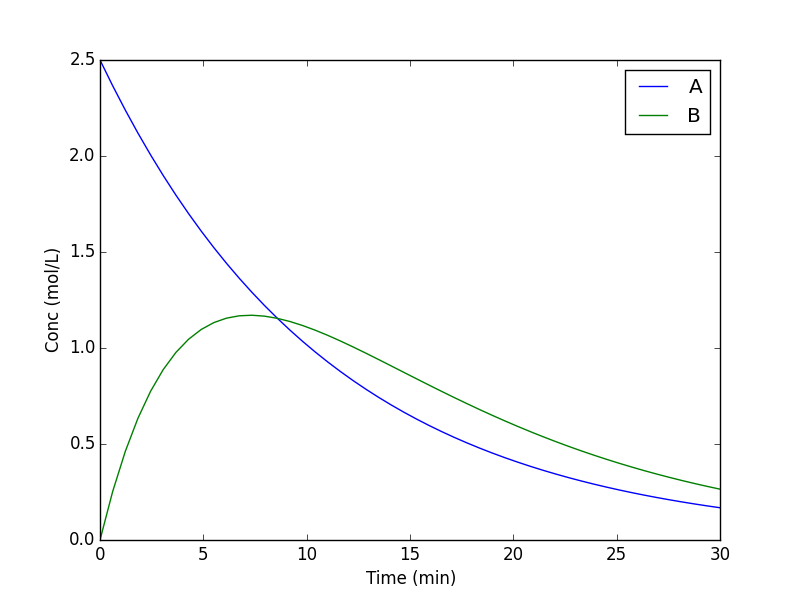
\includegraphics[width=4in]{./images/batch-multiple.png}

\url{org-display-inline-images}
% Emacs 24.4.50.1 (Org mode 8.2.7c)
\end{document}
